\documentclass[12pt,thmsa]{article}\usepackage[]{graphicx}\usepackage[]{color}
% maxwidth is the original width if it is less than linewidth
% otherwise use linewidth (to make sure the graphics do not exceed the margin)
\makeatletter
\def\maxwidth{ %
  \ifdim\Gin@nat@width>\linewidth
    \linewidth
  \else
    \Gin@nat@width
  \fi
}
\makeatother

\definecolor{fgcolor}{rgb}{0.345, 0.345, 0.345}
\newcommand{\hlnum}[1]{\textcolor[rgb]{0.686,0.059,0.569}{#1}}%
\newcommand{\hlstr}[1]{\textcolor[rgb]{0.192,0.494,0.8}{#1}}%
\newcommand{\hlcom}[1]{\textcolor[rgb]{0.678,0.584,0.686}{\textit{#1}}}%
\newcommand{\hlopt}[1]{\textcolor[rgb]{0,0,0}{#1}}%
\newcommand{\hlstd}[1]{\textcolor[rgb]{0.345,0.345,0.345}{#1}}%
\newcommand{\hlkwa}[1]{\textcolor[rgb]{0.161,0.373,0.58}{\textbf{#1}}}%
\newcommand{\hlkwb}[1]{\textcolor[rgb]{0.69,0.353,0.396}{#1}}%
\newcommand{\hlkwc}[1]{\textcolor[rgb]{0.333,0.667,0.333}{#1}}%
\newcommand{\hlkwd}[1]{\textcolor[rgb]{0.737,0.353,0.396}{\textbf{#1}}}%
\let\hlipl\hlkwb

\usepackage{framed}
\makeatletter
\newenvironment{kframe}{%
 \def\at@end@of@kframe{}%
 \ifinner\ifhmode%
  \def\at@end@of@kframe{\end{minipage}}%
  \begin{minipage}{\columnwidth}%
 \fi\fi%
 \def\FrameCommand##1{\hskip\@totalleftmargin \hskip-\fboxsep
 \colorbox{shadecolor}{##1}\hskip-\fboxsep
     % There is no \\@totalrightmargin, so:
     \hskip-\linewidth \hskip-\@totalleftmargin \hskip\columnwidth}%
 \MakeFramed {\advance\hsize-\width
   \@totalleftmargin\z@ \linewidth\hsize
   \@setminipage}}%
 {\par\unskip\endMakeFramed%
 \at@end@of@kframe}
\makeatother

\definecolor{shadecolor}{rgb}{.97, .97, .97}
\definecolor{messagecolor}{rgb}{0, 0, 0}
\definecolor{warningcolor}{rgb}{1, 0, 1}
\definecolor{errorcolor}{rgb}{1, 0, 0}
\newenvironment{knitrout}{}{} % an empty environment to be redefined in TeX

\usepackage{alltt}
\usepackage[french,english]{babel}
\usepackage[ansinew]{inputenc}
\usepackage[T1,OT1]{fontenc}
\usepackage{graphicx}
\usepackage{amsmath,amssymb,listings}
\usepackage{alltt,algorithmic,algorithm}
\usepackage{multicol}
\usepackage{cite}
\usepackage{fancyhdr}
\usepackage{setspace}
\usepackage{array}
\usepackage{amsfonts}
\usepackage{latexsym}
\usepackage{epsf}
\usepackage{umlaute}
\usepackage{setspace}
\usepackage{amsthm}
\usepackage{enumerate}


\setlength{\textwidth}{160mm}
\setlength{\textheight}{230mm}
\setlength{\oddsidemargin}{-5mm}
\setlength{\topmargin}{-10mm}

% to get rid of the numbers in the bibliography:
\makeatletter
\def\@biblabel#1{}
\makeatother



\title{Assignement 2}
\IfFileExists{upquote.sty}{\usepackage{upquote}}{}
\begin{document}


\noindent \textsc{University of Geneva}     \hfill \textsc{Bachelor in Economics and Management} \\
\textbf{Probability 1}                      \hfill \textsc{Bachelor in International Relations} \\
Dr. Daniel \textsc{Flores Agreda}                 \hfill Spring 2021  \\
ASSIGNMENT 02                               \hfill   March 6th



\noindent
\makebox[\linewidth]{\rule{\textwidth}{0.4pt}}\\[1.5ex]





\section*{Exercise 1}

\begin{enumerate}
\item Let $ A $, $ B $ and $ C $ be three sets as shown in the following Venn diagram.\\
\begin{figure}[h!]
\begin{center}
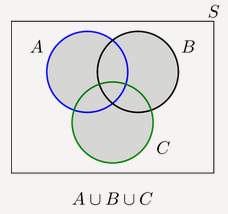
\includegraphics[scale=1]{Capture.png}
\end{center}
\end{figure}
\newline
For each of the following sets, draw a Venn diagram and shade the area representing the given set.
\begin{enumerate}[a)]
\item $ A \cup B \cup C $
\item $ A \cap B \cap C $
\item $ A \cup (B \cap C) $
\item $ A - (B \cap C) $
\item $ A \cup (B \cap C)^{c} $
\end{enumerate}


\item Using the Venn Diagrams, verify the following identities.
\begin{enumerate}[a)]
\item Transitive Property: If $A \subset B$ and $B \subset C$, then $A \subset C$. \\
\item Distributive Property: $A \cup (B \cap C) = (A \cup B) \cap (A \cup C)$, $A \cap (B \cup C) = (A \cap B) \cup (A \cap C) $ \\
\item De Morgan's Laws: $(A \cap B)^c = A^c \cup B^c $, $(A \cup B)^c = A^c \cap B^c $\\
\item $ A=(A \cap B) \cup (A-B) $
\item If $ A $ and $ B $ are finite sets, we have $ |A \cup B|=|A|+|B|-|A \cap B| $
\subitem Note that the symbol $ | . | $ indicates the cardinality, i.e. the measure of the ``number of elements of the set".
\end{enumerate}

\item Determine whether each of the following sets is countable or uncountable:
\begin{enumerate}[a)]
\item $ A=\{(x,y)|x \in N, y \in Z\} $
\item $ B=(0, 0.1] $
\item $ C=\{\frac{1}{n}|n \in N\} $
\item $ D=\mathbb{Q} $
\end{enumerate}

Solutions:\\
$ A=\{(x,y)|x \in N, y \in Z\} $ is countable because it is a cartesian product of two countable sets, i.e. $ A=N \times Z $\\
$ B=(0, 0.1] $ is uncountable since it is an interval of the form $ (a,b] $, where $ a < b $.\\
$ C=\{\frac{1}{n}|n \in N\} $ is countable since it is a one-to-one correspondence with the set of natural numbers. In particular, you can list all the elements in the set $C$, $ C=\{1, \frac{1}{2}, \frac{1}{3}, ...\} $\\
$ D=\mathbb{Q} $  is countable since rational numbers can be expressed as the fraction of two integers.  It is a one-to-one correspondence with the set of natural numbers.




\end{enumerate}

\section*{Exercise 2}


We consider an urn with $N$ marbles containing $r$ reds and $N-r$ blacks. We draw $n$ marbles randomly without repetition.
\begin{enumerate}
  \item How many possible outcomes do we have?
  \item How many of these outcomes would include $k$ red marbles.
  \item Deduce the probability of choosing $k$ red marbles.
\end{enumerate}

Solutions:
\begin{enumerate}
\item $C^{n}_{N}$
\item $C^{k}_{r} C^{n-k}_{N-r}$
\item P(choosing k red marbles)=$\dfrac{\text{number of outcomes including k red marbles}}{\text{number of possible outcomes}}=\dfrac{C^{k}_{r} C^{n-k}_{N-r}}{C^{n}_{N}}$
\end{enumerate}

\section*{Exercise 3}
There are 3 pairs of shoes of different color in the drawer. We randomly draw 2 shoes without repetition;
determine the probability associated with each of the following events:

 \begin{center}
 \begin{tabular}{l}
 $A$ : `they belong to the same pair';  \\
 $B$ : `there is a right shoe and a left shoe'.
 \end{tabular}
 \end{center}

\noindent Solutions:\\
In the drawer there are three pairs of shoes of different color. The number of possible outcomes must first be counted when two random shoes are drawn.\\
\\
We use the following notation:
\begin{itemize}
\item G1: Left shoe of the first pair;
\item G2: Left shoe of the second pair;
\item G3: Left shoe of the third pair;
\item D1: Right shoe of the first pair;
\item D2: Right shoe of the second pair;
\item D3: Right shoe of the third pair.
\end{itemize}
\medskip
All possible outcomes are:
\begin{itemize}
\item (G1 D1), (G1 D2), (G1 D3), (G1 G2), (G1 G3),
\item (G2 D1), (G2 D2), (G2 D3), (G2 G3),
\item (G3 D1), (G3 D2), (G3 D3),
\item (D1 D2), (D1 D3),
\item (D2 D3).
\end{itemize}
\medskip
There are 15 possible outcomes. That is $C^{2}_{6}$.\\
\\
Note:
Both events A and B do not take into account the order in which we
draw the shoes. So we simplify the basic set without taking order in count\footnote{It is quite correct to count the fundamental set by taking the order into account, but it is not necessary in this case to identify events $A$ and $B$.}. For example, drawing G1 then D1 is the same event as drawing D1 then G1, noted (G1 D1).\\
\newpage

To calculate the probability of the events A and B, as all the elements of our fundamental set are equiprobable, we use:
\begin{center}$P(A)= \displaystyle \frac{\text{Number of favourable outcomes}}{\text{Number of possible outcomes}}=\frac{\rm CF}{\rm CP}.$
\end{center}
\medskip

We count the number of favourable cases corresponding to each event:
\begin{itemize}
\item Event $A$ `belong to the same pair':
\begin{center} (G1 D1), (G2 D2), (G3 D3); \textbf{3 favourable cases}; \end{center}
\item Event $B$ `there is a right shoe and a left shoe':
\begin{center}(G1 D1), (G1 D2), (G1 D3), (G2 D1), (G2 D2), (G2 D3), (G3 D1), (G3 D2),\\ (G3 D3); \textbf{9 favourable cases}.\end{center}
\end{itemize}
\medskip

So
\begin{center}
$ \begin{array}{c}
P(A)= \displaystyle \frac{\rm CF}{\rm CP}=\frac{3}{15}=\frac{1}{5};
\\
\\
P(B)=\displaystyle \frac{\rm CF}{\rm CP}=\frac{9}{15}=\frac{3}{5}.
\end{array}$
\end{center}


\section*{Exercise 4}
Let $A$ be a die whose faces display the values 2, 2, 4, 4, 9, 9.  Let $B$ be a die whose faces display the
values 1, 1, 6, 6, 8, 8. We roll the two dice.


\begin{enumerate} %[(a)]
\item Write all the possible outcomes.
\begin{center} $S=\{(2;1),(2;6),(2;8),(4;1),(4;6),(4;8),(9;1),(9;6),(9;8)\}$
\end{center}
There are a total of 9 equiprobable events (possible cases). \footnote{In this exercise, we could also define the fundamental set in more detail if we consider that among the 6 faces of two dice. For example, the value `4' actually includes two different cases: The first face of A `4' could be noted 4.1 and the second face of A `4' could be noted 4.2. In this case, we would have:
\begin{center}
$S = $ \\ $ \{(2.1;1.1),(2.1;1.2),(2.2;1.1),(2.2;1.2)$\\$(2.1;6.1),(2.1;6.2),(2.2;6.1),(2.2;6.2)$\\$(2.1;8.1),(2.1;8.2)
,(2.2;8.1),(2.2;8.2)$\\$...$\\$(9.1;8.1),(9.1;8.2),(9.2;8.1),(9.2;8.2)\}$
\end{center}
a fundamental set of 36 equiprobable elements. But as we see, each element of type (2,1) is obtained in 4 different ways. So we can rewrite the fundamental set in a compact way as we did before, because the possible cases remain equiprobable.}


\item What is the probability that the result of $A$ is greater than the result of $B$?

We count the number of favorable outcomes corresponding to the event  `$A> B$':\\
(2; 1), (4; 1), (9;1), (9;6), (9;8); 5 favorable cases. So
\begin{center} $P(A>B)=\displaystyle \frac{\rm CF}{\rm CP}=\frac{5}{9}.$
\end{center}


\item What is the probability that the sum of the two dice equals $10$?


We count the number of favorable outcomes corresponding to the event  `$A$ + $B$ $= 10$':
 (2;8), (4;6), (9;1). So
\begin{center} $P(A+B=10)=\displaystyle \frac{\rm CF}{\rm CP}=\frac{3}{9}=\frac{1}{3}.$
\end{center}
\end{enumerate}


\section*{Exercise 5}
A cafeteria offers a three-course menu. We choose a main course, a starch and a
dessert. The possible choices are given below:

\begin{itemize}
\item `Main course': Chicken (C) or roast beef (B);
\item `Starch': Pasta (P) or rice (R) or potatoes (T);
\item `Dessert': Ice cream(I) or jelly (J) or apple pie (A) or peach pie (P).
\end{itemize}

A person chooses a dish from each category.

\begin{enumerate}
\item How many possible menus are there in the basic set?\\
The basic set is:
\begin{align*}
S= \{ & (C;P;I), (C;P;J), (C;P;A), (C;P;P), (C;R;I), (C;R;J), (C;R;A), (C;R;P),\\ & (C;T;I), (C;T;J), (C;T;A), (C;T;P),  (B;P;I), (B;P;J), (B;P;A), (B;P;P),\\ & (B;R;I), (B;R;J), (B;R;A), (B;R;P),(B;T;I), (B;T;J), (B;T;A), (B;T;P) \}.
\end{align*}
24 possible menus. ($C^{1}_{2}C^{1}_{3}C^{1}_{4}=24$)
\medskip

\item Let $A$ be the event: `we choose ice cream'. How many menus are there in $A$?\\
In event $A$, we take dessert `ice cream' with certainty. So the set of possible outcomes in this case is:
\begin{align*}
S_A = \{ (C;P;I),(C;R;I), (C;T;I), (B;P;I),(B;R;I), (B;T;I)   \}.
\end{align*}
So, 6 menus are possible in event $A$. ($C^{1}_{2}C^{1}_{3}=6$)
\medskip

\item  Let $B$ be the event: `we choose the chicken'. How many menus are there in $B$?\\
In event $B$, we take the chicken with certainty. The set of possible menus then becomes:
\begin{align*}
S_B = \{  & (C;P;I), (C;P;J), (C;P;A), (C;P;P), (C;R;I), (C;R;J), \\ & (C;R;A), (C;R;P), (C;T;I), (C;T;J), (C;T;A), (C;T;P) \}
\end{align*}
So, 12 menus belong to Event $B$. ($C^{1}_{3}C^{1}_{4}=12$)
\medskip

\item Give all the possible menus of the event $A \cap B$.\\
In event $A\cap B$ we take chicken and ice cream. Hence the set of possible menus becomes:
\begin{align*}
S_{A \cap B} = \{ (C;P;I),(C;R;I),(C;T;I)  \}.
\end{align*}
3 possible menus are in $A\cap B$. ($C^{1}_{3}=3$)
\medskip

\item Let $C$ be the event: `we choose rice'. How many menus are there in $C$?\\
 In event $C$, rice is taken with certainty. So, the set of possible menus is:
\begin{align*}
S_C = \{  (C;R;I),(C;R;J),(C;R;A),(C;R;P), (B;R;I),(B;R;J),(B;R;A),(B;R;P) \}.
\end{align*}
There are 8 possible menus. ($C^{1}_{2}C^{1}_{4}=8$)
\medskip

 \item It is assumed that a person randomly selects his menu by associating an equal probability with
all the options for each category. What is the probability that the chosen menu belongs to event $A$?
Answer the same questions for event $B$ and for event $C$.\\
 As each option in each dish is equiprobable, each menu has the same probability of being taken. We define $X$ as the chosen menu. So,
\begin{align*}
P(X \in A) =  \frac{6}{24} = \frac{1}{4}.
\end{align*}
Similarly for events $B$ and $C$ we have:
\begin{align*}
P(X \in B) = \frac{12} {24} = \frac{1}{2}; \\
P(X \in C) = \frac{8}{24} = \frac{1}{3}.
\end{align*}

\end{enumerate}

\newpage

\section*{Exercise 6 (Optional)}
In this problem, you are given descriptions in words of certain events (e.g., at least one of the events A,B,C occurs). For each one of these descriptions, identify the correct symbolic description in terms of A, B, C from Events E1-E7 below. Also identify the correct description in terms of regions (i.e., subsets of the sample space $\Omega$) as depicted in the Venn diagram below. (For example, Region 1 is the part of A outside of B and C.)
\begin{center}
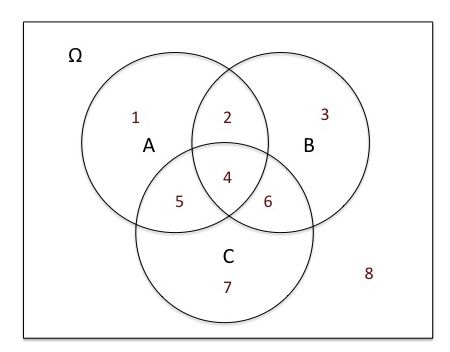
\includegraphics[width = 2in]{images1.jpg}
\end{center}

\noindent Symbolic descriptions: \\
Event E1: $A \cap B \cap C$ covers Region {4}\\
Event E2: $(A\cap B \cap C)^c $ covers Region {1,2,3,5,6,7,8} \\
Event E3: $ A \cap B \cap C^c $ covers Region {2} \\
Event E4: $B \cup (B^c \cap C^c)$ covers Region {1,2,3,4,6,8}\\
Event E5: $A^c \cap B^c \cap C^c $ covers Region {8} \\
Event E6: $(A \cap B) \cup (A \cap C) \cup (B \cap C)$ covers Region {2,4,5,6} \\
Event E7: $(A \cap B^c \cap C^c) \cup (A^c \cap B \cap C^c) \cup (A^c \cap B^c \cap C) $ covers Region {1,3,7}\\

\noindent Which Event or Regions satisfy the following conditions.
\begin{enumerate}
\item At least two of the events A, B, C occur. \\
Region {2,4,5,6} (E6) satisfy this condition.
\item At most two of the events A, B, C occur. \\
Region {1,2,3,5,6,7,8} (E2) satisfy this condition.
\item None of the events A, B, C occurs. \\
Region {8} (E5) satisfy this condition.
\item All three events A, B, C occur. \\
Region {4} (E1) satisfy this condition.
\item Exactly one of the events A, B, C occurs.\\
Region {1,3,7} (E7) satisfy this condition.
\item Events A and B occur, but C does not occur. \\
Region {2} (E3) satisfy this condition.
\item Either event B occurs or, if not, then C also does not occur.\\
Region {1,2,3,4,6,8} (E4) satisfy this condition.


\end{enumerate}

\section*{Exercise 7 (Optional)}

A,B and C take turns flipping a coin, that is: A flips first, then B, then C, then A and so on. The first one get a head wins.
\begin{enumerate}
  \item Define the sample space $S$ of all the possible outcomes.

H: Head, T: Tail\\
$S = \{H,TH, TTH, TTTH, TTTTH, \cdots ,\underbrace{TT\cdots TT}_{\text{n times}}H, \cdots, \underbrace{TT\cdots TT}_{\text{infinite T}}\}$
  \item Define the following events in terms of $S$:
\begin{enumerate}
  \item The event $A$: A wins.

The time that A flips are $1_{st}, 4_{th},7_{th}, \cdots, {(3k+1)}_{th}, \cdots$.\\
$Event A = \{H, TTTH, TTTTTTH, \underbrace{TT\cdots TT}_{3k}H, \cdots \}$
  \item The event $B$: B wins.

The time that B flips are $2_{nd}, 5_{th},8_{th}, \cdots, {(3k +2)}_{th}, \cdots$.\\
$Event B = \{TH, TTTTH, TTTTTTTH, \underbrace{TT\cdots TT}_{3k+1}H, \cdots \}$
  \item $(A \cup B)^c$

$(A \cup B)^c=\{\text{C wins}\}+ \{\text{no one wins}\}$\\
The time that C flips are $3_{rd}, 6_{th},9_{th}, \cdots, {(3k+3)}_{th}, \cdots$.\\
$\{\text{C wins}\} = \{TTH,TTTTTH, TTTTTTTTH, \underbrace{TT\cdots TT}_{3k+2}H, \cdots \}$\\
 $\{\text{no one wins}\} = \{ \underbrace{TT\cdots TT}_{\text{infinite T}}\}$ \\
So $(A \cup B)^c=\{TTH, TTTTTH, TTTTTTTTH, \underbrace{TT\cdots TT}_{3k+2}H, \cdots,\underbrace{TT\cdots TT}_{\text{infinite T}} \}$

\end{enumerate}
\end{enumerate}

\end{document}














